\chapter{پژوهش‌های پیشین}\label{chap2}
\minitoc

در این فصل برخی مدل‌های ارائه شده مرتبط با مسئله گپ‌زن دانش  ارائه و بررسی خواهند شد. در انتها نیز برخی دادگان جمع‌آوری شده در طی سالیان اخیر که می‌توانند برای مساله گپ‌زن دانش مفید واقع شوند معرفی شده اند.

\section{مدل‌های گپ‌زن دانش بنیان}\label{intro}

\subsection{مدل پیشنهاد شده توسط وینیالز}

این مدل در سال ۲۰۱۵ و بر پایه معماری دنباله به دنباله با استفاده از شبکه LSTM 
دو لایه با اندازه 
\trans{Hidden State }{حالت نهان}
۴۰۹۶
ارائه شد
\cite{A_Neural_Conversational_Model}.
این مدل در واقع فاقد منبع دانش خارجی است و صرفا از شبکه آموزش دیده شده روی دادگان آموزشی تشکیل شده است. اما اهمیت ذکر این مدل در اینجا، به دلیل نشان دادن این حقیقت است که حتی مدل‌های فاقد منبع دانش نیز  علاوه بر تقلید 
\trans{دستور زبان}{grammar}
 مکالمه انسانی، قادرند تا مقداری از حقایق جهان را در شبکه خود ذخیره کنند.
 برای مثال،‌ نمونه‌ای از گفتگوی چالشی دانش‌محور عامل انسانی با این مدل در شکل
 \ref{fig:chap2:Vinyals1}
 آورده شده است.

\begin{figure}[h]
	\centering
	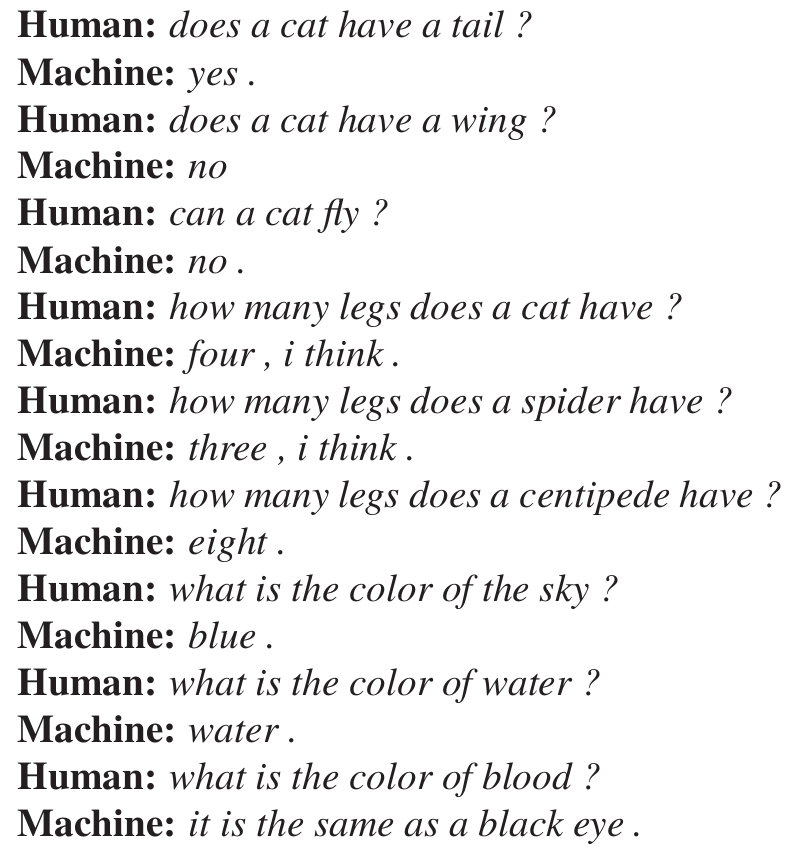
\includegraphics[width=0.75\textwidth]{images/chap2/Vinyals1.png}
	\caption{
		نمونه‌‌ای از گفتگوی چالشی دانش‌محور عامل انسانی با مدل وینیالز
		\cite{A_Neural_Conversational_Model} 
	}
	\label{fig:chap2:Vinyals1}
\end{figure}

همانطور که در شکل
\ref{fig:chap2:Vinyals1}
مشاهده‌ می‌شود مدل در پاسخ به سوالاتی مانند تعدادی پا‌های گربه و یا رنگ آسمان توانسته‌ است به خوبی پاسخ درست را خروجی دهد، حال آن که در موارد دیگری نظیری رنگ آب و یا تعداد پاهای عنکبوت نتوانسته‌است به موفقیت دست پیدا کند.

مدل وینیالز را می‌توان یکی از اولین تلاش‌های موثر در دستیابی به گپ‌زن دامنه باز دانست. این مدل سعی کرد تا با آموزش بر روی دادگان عظیم 
\lr{OpenSubtitle}
به این مهم دست یابد و توانایی این مدل در برخی استنتاج‌‌ها و پاسخگویی به سوالات چالشی دانش‌محور را نیز می‌توان به نوعی از تاثیرات حجم عظیم دادگان‌ آموزشی آن دانست.
\cite{Tiedemann2009NewsFO}
 پژوهش وینیالز علاوه بر موارد فنی مطرح شده، در زمینه آزمایش و ارزیابی مدل خود از آزمایشات جالب توجه و چالش بر‌انگیز  انجام مکالمات چالش برانگیز 
(نظیر آن‌چه که در شکل 
\ref{fig:chap2:Vinyals1}
به نمایش درآمد
)
استفاده کرد که می‌تواند نمونه‌ای‌ مناسب برای ارزیابی مدل‌های بعد از خود باشد. 

\subsection{مدل پیشنهاد شده توسط قزوینی نژاد}
این مدل را می‌توان به نوعی نخستین سامانه گپ‌زن تماما داده محوری دانست که به طور موثر از دانش بیرونی خود استفاده می‌کند
\cite{a_knowledge_grounded}.
انگیزه اصلی این مدل، این بوده است که از آنجایی که بخش عمده‌ای از دانش دنیا در دادگان آموزشی ارائه شده برای مسئله مکالمه حاضر نیستند، در نتیجه سامانه‌های مکالمه حاصل از آموزش روی این دادگان نیز نمی‌توانند عملکرد دانش‌مداری از خود ارائه دهند. از طرفی حتی اگر تمامی دانش دنیای بیرونی را بتوان در یک دادگان آموزشی گنجاند، این دادگان قطعا به حدی غیرقابل تصور بزرگ خواهد بود و قادر به آموزش مدل خود روی آن نیستیم
\cite{a_knowledge_grounded}.
در نتیجه برای حل مشکل دانش بنیان‌کردن سامانه‌ گپ‌زن این مقاله روشی را پیشنهاد داده است که در آن سعی کرده است از تکرار دانش در دادگان آموزشی پرهیز کند و از طرفی بتواند مدل مکالمه پایه را به گونه‌ای تعمیم دهد که قابلیت نمایش دانش رانیز داشته باشد. برای نیل به این هدف، این پژوهش سعی کرده است تا از حقایق موجود در پست‌های شبکه‌های اجتماعی نظیر توییتر و 
\lr{Four-Square} 
استفاده کند و به کمک آن‌ها پاسخ‌های با ارزش اطلاعاتی تولید کند.

به منظور آموزش این مدل گپ‌زن سه مجموعه دادگان جمع‌آوری شده است. دسته اول شامل ۱.۱ میلیون نظرات افراد در شبکه اجتماعی 
\lr{four square}
است که راجع به رستوران‌های آمریکا و کانادا اظهار شده است. این مجموعه جملات در واقع نقش حقایق جهان بیرونی را برای این مدل دارند. دسته دوم ۲۳ میلیون سه‌تایی‌های گفت و گو شده در
توییتر
هستند. این دسته دوم، در واقع نشان ستون فقرات مدل را دارند و برای این فراهم شده اند تا مدل بتواند نحوه کلی چگونگی مکالمه کردن را بیاموزد.
دسته سوم اما حدود ۱ میلیون زوج متشکل از یک توییت و پاسخ به آن هستند که  در مورد یکی از موجودیت‌های مطرح‌شده در مجموعه حقایق مدل (دسته اول دادگان) هستند.

در این مدل ابتدا تمرکز گفتگو تعیین می‌شود. این فرآیند تعیین تمرکز در حالات ساده و ابتدایی می‌تواند به صورت استخراج کلیدواژه‌های خاصی مثل نام شهر‌ها، شرکت‌ها و یا کالا‌ها از گفتگو و یا در حالت پیچیده‌تر به صورت تشخیص موجودیت‌های اسمی
گفتگو، صورت گیرد.
در مرحله بعد جملات مرتبط با تمرکز تعیین‌شده در پایگاه دانش که متشکل از جملات پست‌های کاربران در شبکه‌های اجتماعی توییتر
و
\lr{Four Square}
است مورد جستجو واقع شده و جملات مربوط از پایگاه دانش استخراج و به عنوان مجموعه حقایق ذخیره می‌شوند.
در ادامه تاریخچه گفتگو توسط یک رمزگذار که از نوع شبکه بازگشتی است به یک بردار با طول ثابت تصویر می‌شود. در ادامه برای شیوه و چگونگی رمزکردن حقایق و دخیل کردن آن‌ها، این مقاله از ایده 
\trans{شبکه‌های حافظه‌ای}{memory networks}
استفاده کرده است
\cite{weston2014memory}
. اگر
$u \in R^d$
را برداری 
حاصل از اعمال رمزنگار بازگشتی بر روی تاریخچه گفتگو فرض کنیم آنگاه روابط نظری مورد استفاده مدل برای دخیل کردن حقایق به شرح زیر هستند:

\begin{equation}
\label{eq:a_knowledge_ground}
\begin{split}
m_i &= Ar_i , A \in R^{d \times v} \\
c_i &= Cr_i , A \in R^{d \times v} \\
p_i &= softmax(u^T m_i) \\ 
o_i &= \sum_{i=1}^{k} p_i c_i \\
\hat{u} &= u + o
\end{split}\end{equation}

لازم به ذکر است که در عبارات فوق،
$r_i$
بردار
\trans{کیسه کلمات}{Bag of Words}
 حقیقت
$i$
ام است.
در صورتی که بخواهیم عبارت فوق را تفسیر کنیم، می‌توانیم این گونه بنگریم که بردار
$u$
در نقش یک بردار پرس و جو در یک مکانیزم شبیه به توجه، بر روی بردارهای 
$m$
مورد جستجو قرار می‌گیرد و در نهایت خروجی رمزگذار حقیقت، ترکیبی خطی (که ضریب هر جمله متناسب با میزان شباهت آن با بردار خلاصه تاریخچه گفتگو است)
از بردار‌های
$c$
متعلق به حقایق مختلف است.
سپس این بردار خروجی
$o$
با بردار خلاصه تاریخچه گفتگو جمع می‌شود و به عنوان حالت نهان اولیه به
رمزگشای پاسخ داده می‌شود که وظیفه آن تولید پاسخ برای نوبت بعدی گفتگو است. نمایی از معماری مدل ارائه شده توسط قزوینی‌نژاد در شکل
\ref{fig:chap2:qazvini-arch}
آمده است.

 \begin{figure}[H]
	\centering
	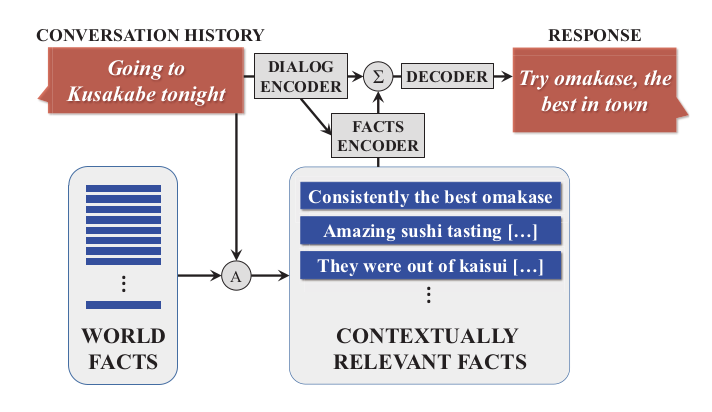
\includegraphics[width=0.75\textwidth]{images/chap2/qazvini-arch.png}
	\caption{نمایشی از معماری مدل مکالمه ارائه شده توسط قزوینی‌نژاد
		\cite{a_knowledge_grounded}}	
	\label{fig:chap2:qazvini-arch}
\end{figure}

ابتکار قابل ذکر این مقاله اما در چگونگی آموزش مدل است. به این صورت که با توجه به سه‌تایی موجود تاریخچه گفتگو، حقایق مرتبط با هر تاریخچه و پاسخ مطلوب تعدادی وظیفه منحصر به فرد تعریف شده‌اند. سپس مجموعه‌ای از ترکیب این وظایف با یکدیگر مشخص شده و مدل هر بار بر اجتماعی از این وظایف به صورت 
\trans{یادگیری چندوظیفه‌ای}{Multitask Learning}
آموزش می‌بیند. در نهایت نشان داده می‌شود که ترکیب این وظایف چگونه باعث بهبود عملکرد مدل می‌شود
\cite{a_knowledge_grounded}
.
در آخر، این پژوهش برای ارزیابی مدل پیشنهادی خود از دو دسته ارزیابی‌های
\trans{ذهنی}{subjective}
و
\trans{عینی}{objective}
استفاده می‌کند.
برای ارزیابی عینی از معیار‌های
\lr{BLEU}
و
\lr{Perplexity} 
بر روی پاسخ‌های تولیدشده استفاده می‌شود
\cite{papineni-etal-2002-bleu}
. برای ارزیابی ذهنی نیز، این پژوهش از نظرسنجی انسانی بر روی دو ملاک میزان مناسب بودن پاسخ تولیدشده و میزان آموزنده و با اطلاعات‌بودن پاسخ بهره برده است.


\subsection{مدل جادوگر ویکی‌پدیا} 

یکی از چالش‌های بزرگ بر سر راه گپ‌زن‌های دانش بنیان، عدم وجود دادگان و 
\trans{سنجه}{benchmark}
برای این وظیفه است. 
دینان در این پژوهش
در ابتدا به وسیله تعریف یک سناریو مشخص و 
\trans{جمع بسپاری}{crowdsourcing}
دادگانی را برای مسئله دانش بنیان کردن گپ‌زن‌ها جمع آوری نموده است و سپس با بهره‌گیری از ترنسفورمر‌ها 
معماری را ارائه کرده است که قابلیت بازیابی دانش و تولید پاسخ مشروط به دانش را داراست
\cite{wizard}. 

سناریویی که برای جمع آوری دادگان در نظر گرفته شده است به این شرح است که ابتدا موضوعی به صورت تصادفی تعیین می‌شود و قرار است که در ادامه دو نفر درباره این موضوع با یکدیگر گفتگو کنند، به علاوه ممکن است این موضوع در طی گفتگو گسترده‌تر شود یا این که به موضوعات مرتبطش متمرکز شده و تغییر پیدا کند. این دو نفر دو نقش متفاوت را در این سناریو بازی می‌کنند به این معنی که یک نفر نقش شاگرد کنجکاو را دارد و بیشتر در پی کشف اطلاعات در مورد موضوع مورد گفتگو و عمیق کردن بحث در مورد آن است و طرف مقابل در نقش استاد است که در مورد موضوع مورد گفتگو اطلاعات کاملی را دارد و هدفش انتقال اطلاعات در مورد موضوع به طرف مقابل است
\cite{wizard}.

روند یک گپ‌ میان استاد و شاگرد به این صورت است که ابتدا یکی از طرفین به تصادف انتخاب شده و موضوعی را انتخاب می‌کنند و راجع به آن سخن می‌گوید. سپس هر موقع که شاگرد پیامی را به استاد بفرستد، به استاد لیستی از دانش‌های مربوط به گفتگوی فعلی نمایش‌ داده می‌شود؛ استاد یکی از جملات را انتخاب می‌کند و با توجه به آن پاسخی به شاگرد می‌دهد(استاد همچنین می‌تواند هیچ جمله‌ای را انتخاب نکند).
این مکالمه در نهایت پس از حداقل چند نوبت رد و بدل شدن پیام به صورت تصادفی پایان می‌پذیرد.
حال پس از جمع‌ آوری دادگان هدف جایگزینی نقش استاد با یک سامانه مکالمه‌گر است
\cite{wizard}
.

به این منظور این مقاله معماری را ارائه کرده است که از سه بخش تشکیل شده است. بخش اول مسئول بازیابی دانش از صفحات ویکی‌پدیا، بخش دوم مسئول مطالعه و توجه به مجموعه دانش‌های بازیابی شده و در نهایت بخش سوم نیز مسئول تولید کردن پاسخ نوبت بعدی گفتگو هستند.

برای بخش اول از یک 
\trans{پیمانه}{Module}
\trans{بازیابی اطلاعات}{Information Retreival}
 ارائه شده در 
مدل ارائه شده توسط دنگی چن در ۲۰۱۷
استفاده شده است که وظیفه آن  پیدا کردن صفحات مرتبط با گفتگو از ویکی‌پدیا است
\cite{drqa_paper}
. پس از پیدا شدن صفحات مرتبط پاراگراف اول آن صفحات (که معمولا خلاصه‌ای از آن صفحه هستند) برداشته می‌شوند و به جملاتشان می‌‌شکنند. سپس به ابتدای هر جمله عنوان صفحه آن اضافه شده و جملات برای استفاده در مرحله بعدی ذخیره می‌شوند. 

هدف بخش دوم از معماری یعنی قسمت توجه به دانش، این است که با توجه به تاریخچه گفتگو و جملات استخراج شده از بخش اول، جمله اصلی مرتبط با گفتگو را حدس زده و آن را تعیین کند. این بخش از معماری از یک ترنسفورمر بهره برده است به این شکل که تاریخچه گفتگو و هر یک از جملات استخراج شده در بخش اول با یک ترنسفومر مشابه ولی به صورت جدا و مستقل از هم به یک بردار با طول ثابت رمز می‌شوند. سپس استفاده از ضرب داخلی میزان مشابهت بردار رمز  گفتگو با بردارهای رمز جملات دانش مشخص می‌شود. سپس این میزان مشابهت‌ها از یک لایه 
\lr{softmax}
عبور کرده و با توجه به خطای 
\lr{cross-entropy}
و همچنین جمله‌ای که در دادگان آموزشی به عنوان جمله مرتبط در هنگام تولید پاسخ توسط استاد انتخاب شده است، میزان خطا و تابع هزینه آن مشخص می‌شود.

 در این قسمت مقاله دو رویکرد متفاوت را برای پیاده‌سازی بخش دوم و سوم اتخاذ کرده است. در رویکرد اول که آموزش انتها به انتها است، بردار‌های رمز  تاریخچه گفتگو و جمله دانشی که بیشترین مشابهت با آن را دارد با یکدیگر الحاق می‌شوند و در بخش سوم معماری به یک ترنسفورمر رمزگشا داده می‌شوند و کل بخش دوم و سوم با یکدیگر آموزش می‌بینند.
تابع هزینه‌ای هم که برای آموزش کل این دو بخش مورد استفاده قرار می‌گیرد عبارت زیر است.


\begin{equation}\begin{split}
\mathcal{L} = (1- \lambda ) \mathcal{L}_{NIL} + (\lambda) \mathcal{L}_{knowledge}
\end{split}\end{equation}

که در عبارت بالا
$\mathcal{L}_{NIL}$
میزان خطای رمزگشا به هنگام تولید پاسخ
،
$\mathcal{L}_{knowledge}$
میزان خطای بخش توجه به دانش برای انتخاب جمله صحیح مرتبط
و
$\lambda$
نیز یک ضریب تنظیم‌گر بین خطای انتخاب دانش و تولید پاسخ درست هستند.

اما در رویکرد دوم که آموزش دو مرحله‌ای بخش دوم و سوم است، هر کدام از بخش ‌های دوم و سوم جداگانه آموزش می‌بینند. در این رویکرد پس از انتخاب جمله دانش مرتبط، این جمله و تاریخچه گپ دوباره و با هم با یک ترنسفورمر رمز می‌شوند و سپس وارد ترنسفورمر رمزگشا می‌شوند. از آن جایی که رخدادن خطا در بخش دوم می‌تواند موجب انتشار خطایی قابل توجه برای بخش سوم شود و به نوعی حتی این نوع آموزش دادن دو مرحله‌ای موجب
\trans{بیش‌برازش}{Overfitting}
 بخش سوم روی بخش دوم شود، این مقاله ایده‌ی 
 \trans{حذف تصادفی}{Dropout}
 روی دانش را مطرح کرده است، که در آن به مانند ایده حذف تصادفی
،بخش سوم در مواقعی بایستی بدون دانستن جمله مرتبط   پاسخ صحیح را بتواند تولید کند
\cite{wizard}.

  جهت فهم و درک بهتر نمایی از معماری این دو رویکرد در شکل
\ref{fig:chap2:wizard-arch}
آمده است.

 \begin{figure}[H]
	\centering
	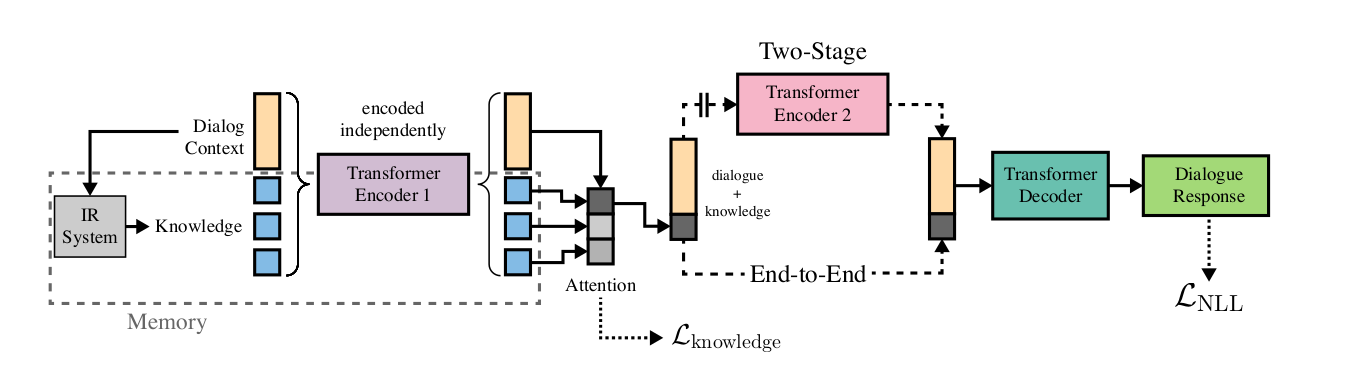
\includegraphics[width=1\textwidth]{images/chap2/wizard_arch.png}
	\caption{نمایشی از معماری مدل مکالمه جادوگر ویکی‌پدیا
		\cite{wizard}}	
	\label{fig:chap2:wizard-arch}
\end{figure}

این پژوهش برای ارزشیابی مدل خود دو رویکرد را دو نوع نگاه را مد نظر قرار داده است. در یک رویکرد عملکرد هر یک از سه بخش را به صورت جداگانه مورد بررسی قرار داده است ( با شرط این که بدانیم ورودی وارد به هر بخش کاملا صحیح است و خطایی از بخش قبل به آن وارد نشده است). در این رویکرد برای ارزیابی بخش دوم از معیارهای بازخوانی و امتیاز 
\lr{f1}
همپوشانی
بین 
\trans{یک‌تایی}{unigram}
‌های بین جمله درست و جمله انتخاب شده، استفاده شده است. همچنین برای بخش سوم نیز از معیار‌های 
امتیاز 
\lr{f1}
همپوشانی
بین 
یک‌تایی
‌های بین جمله درست و جمله تولید شده
و امتیاز ارزیابی انسانی جملات تولید شده استفاده شده است.


\subsection{مدل گپ موضوعی}

دادگان فعلی وظیفه مکالمه مبتنی بر دانش،‌ در حین فرآیند جمع آوری دادگان،‌ برای مکالمه‌گرها نقش‌های مشخصی را تعریف کرده اند.
\footnote{برای مثال در فرآیند جمع آوری دادگان جادوگر ویکی‌پدیا یک مکالمه‌گر نقش دانای کل و دیگری نقش جوینده دانش را به عهده می‌گیرند.}
 این دادگان همچنین، سناریو‌هایی را که در آن مکالمه‌گرها به سمت عمق یک  موضوع حرکت کنند و یا این که در حین مکالمه موضوع گفتگو را تغییر دهند، در نظر نگرفته‌اند. این پژوهش ابتدا سعی در جمع‌آوری دادگانی دارد که چالش‌های مطرح شده را رفع کند و سپس اقدام به طراحی و آموزش یک مدل روی دادگان جمع آوری شده کرده است
 \cite{Topical_Chat}.

در طی این پژوهش حدود یازده هزار مکالمه انسان با انسان با میزان گستردگی هشت موضوع، جمع آوری شده است. در طی مکالمه به هر یک از طرفین یک مجموعه متن خواندنی داده شده است که این مجموعه خواندنی بین دو طرف می‌تواند متقارن یا نامتقارن باشد. سپس از هر یک از طرفین خواسته ‌شده است که یک مکالمه منسجم و جذاب را شکل با توجه به مجموعه متن‌هایی که در پیش خود دارند، شکل دهند. 
در طی این پژوهش همچنین به عنوان سنجه،‌چندین مدل با معماری رمزگذار و رمزگشا را نیز آموزش داده شده اند. در ادامه روند این پژوهش به صورت جزیی‌تر تشریح می‌شود. 

همانطور که گفته شد در طی انجام یک مکالمه دو مجموعه از اسناد به دو طرفین مکالمه داده می‌شود. این دو مجموعه اسناد در صورتی که دقیقا یکسان باشند، متقارن و در غیر این صورت نامتقارن نامیده می‌شوند. سپس مکالمه بین دو طرف با فرض این که هیچ یک از طرفین نقش مشخص معلم یا دانش آموز را ندارند آغاز می‌شود. این مدل جمع‌آوری دادگان را می‌توان تعمیمی از مدل جمع آوری دادگان جادوگر ویکی‌پدیا دانست. همچنین تنظیمات به کار رفته در این رویکرد جمع آوری دادگان را نیز شبیه‌سازی بهتری از مکالمه در دنیای واقعی را بازتاب می‌کند. چه آن که در دنیای واقعی نیز دانشی که طرفین مکالمه نسبت به موضوع دارند و دانش دیگری که جویای دانستن آن از فرد مقابلند،‌ می‌تواند نسبت به طرف مقابل نامتقارن باشد. 

برای ساختن مجموعه‌های مطالعه، یک پایگاه دانش ساخته می‌شود که دارای سه جز موجودیت‌ها، حقیقت‌ها و مقالات است. در ضمن هشت موضوع پوشاک، سیاست، کتاب‌ها، سرگرمی‌های عمومی، موسیقی، علم و تکنولوژی و فیلم‌ها هم در نظر گرفته می‌شوند.
سپس سیصد موجودیت محبوب از این هشت موضوع انتخاب می‌شوند. 
در مرحله بعد برای هر یک از موجودیت‌ها پاراگراف اول و خلاصه صفحه ویکی‌پدیا 
متعلق به آن موجودیت و هشت تا ده مطلب جالب مربوط به آن موجودیت که از طریق جمع‌بسپاری روی ردیت انتخاب شده‌است، جمع‌آوری می‌شوند و به عنوان حقیقت‌ها ذخیره می‌شوند. 
در مرحله بعد، مقالاتی از واشنگتن پست که حداقل سه موجودیت ازموجودیت‌های ذخیره شده را در خود مورد اشاره قرار داده‌اند تحت عنوان مجموعه مقالات ذخیره می‌شوند.

در مرحله بعدی و هنگام آغاز هر مکالمه یک مقاله از مقاله‌های واشینگتن پست به تصادف انتخاب می‌شود  و سه موجودیت پر تکرار در این مقاله نیز استخراج می‌شوند. 
 سپس یکی از چهار تنظیمات متقارن یا نامتقارن بودن مجموعه مطالعه طرفین نیز به تصادف انتخاب می‌شود.
در تنظیمات A، هر دو طرف مقاله‌ی واشنگتن پست و پاراگراف اول  ویکی پدیا را در مجموعه مطالعه خود دارند. از سویی یک طرف نصف اول حقایق مربوط به سه موجودیت را دریافت می‌کند و طرف دیگر نیز نصف دوم حقایق مربوط به سه موجودیت انتخاب شده را دریافت می‌کند.
تنظیمات B مشابه تنظیمات قبلی است با این تفاوت که هر دو مجموعه حقایق یکسانی را دریافت می‌کنند اما یک طرف پاراگراف اول  صفحه ویکی پدیا مربوط به سه موجودیت و طرف دیگر خلاصه صفحه ویکی پدیا مربوط به سه موجودیت را دریافت می‌کنند.
در تنظیمات C هر دو مکالمه‌گر پارگراف اول ویکی‌پدیا مربوط به سه موجودیت و همچنین چهار یا پنج حقیقت یکسان مربوط به هر موجودیت را دریافت می‌کنند اما مقاله واشینگتن پست به آن‌ها داده نمی‌شود. در تنظیمات D نیز هر دو طرف مکالمه مجموعه یکسانی شامل مقاله واشنگتن پست، چهار یا پنج حقیقت مربوط به سه موجودیت و پاراگراف اول صفحات ویکی پدیا مربوط به سه موجودیت را دریافت می‌کنند. تنظیمات A و B تنظیمات نامتقارن و تنظیمات C و D تنظیمات متقارن نامیده می‌شوند.

در این پژوهش دو مدل پیشنهاد شده اند که هر دو مبتنی بر معماری ترنسفورمر هستند. در مدل اول تاریخچه گفتگو که از الحاق نوبت‌های گفتگو به دست آمده است به عنوان ورودی به قسمت رمزگذار ترنسفورمر داده می‌شود و انتظار می‌رود تا در خروجی جمله پاسخ تولید شود.
در مدل دوم اما ابتدا یک جمله 
$K'$ 
به عنوان جمله هدف از جملات حاضر در مجموعه مطالعه انتخاب می‌شود. در صورتی که نوبت‌ بعدی گفتگو که بایستی تولید شود 
$X_{j+1}$
باشد، 
$K'$
این گونه انتخاب می‌شود که:
\\
\begin{gather} \label{eq:topicalchat_knowledge_sel}
k' = \arg\max_{k_i}{
(\frac{x_{j+1}.k_i}{\lVert  x_{j+1}  \rVert 
	\lVert  k_i  \rVert})
}
\end{gather}
\\
که در فرمول 
\ref{eq:topicalchat_knowledge_sel}
نماد‌
$k_i$
بردار کیسه کلمات جمله i ام از منبع دانش و نماد
$x_{j+1}$
بردار کیسه کلمات جمله 
$X_{j+1}$
می‌باشد.
سپس 
$k'$
و تاریخچه گفتگو هر دو با یک رمزگذار مشترک رمز می‌شوند و سپس با هم الحاق می‌شوند و به یک رمز‌گشای ترنسفومر داده می‌شوند و در نهایت این رمزگشا پاسخ را تولید می‌کند. 

نکته جالب توجه و البته عجیب این مدل در این است که در آن مسئله پیدا کردن جمله هدف یک مساله باز و حل نشده است؛ چرا که روش پیشنهاد شده نیز مشروط به داشتن عبارت بعدی گفتگوست که در زمان تست این کار ناممکن است. به همین دلیل مدل پیشنهاد شده توسط این پژوهش، کم ارزش به نظر می‌رسد و اهمیت این پژوهش را می‌توان در نحوه جمع آوری دادگان آن دانست.


\subsection{مدل گپ‌زن دوازه‌گانه}
در این پژوهش، هدف نهایی تولد گپ‌زنی است که بتواند در تمامی دامنه‌ها و موضوعات گفتگو کند و از طرفی خصوصیات یک مکالمه انسانی را نیز به خوبی نشان دهد و در کل بتواند کاربر را مشتاق و درگیر با مکالمه با خود کند. به این منظور،‌در این پژوهش چندین توانایی موردنیاز و لازم برای رسیدن به گپ‌زنی که بتواند عامل انسانی را مشتاق به مکالمه با خود کند در نظر گرفته شده است. این چندین توانایی عبارتند از توانایی شخصیت داشتن گپ‌زن، توانایی انتقال احساسات وعواطف  در گفتگو توسط گپ‌زن، توانایی پرسیدن سوال از سوی گپ‌زن (به منظور روشن‌کردن ابهامات گفتگوی کاربر انسانی)، توانایی درک و بحث در مورد تصاویر، توانایی بحث در موضوعات و موقعیت‌های متفاوت و البته توانایی سوال‌دادن با توجه به منابع دانش خارجی
\cite{dodecathlon_paper}.

البته لازم به ذکر است که از که هیچ وظیفه و دادگان مشخصی وجود ندارد که همه توانایی بالا را بتواند دربرگیرد. اما در عوض تعداد زیادی دادگان و مسائل جدای از هم،‌وجود دارند که هر کدام دنبال ارضای یکی از توانایی‌های مذکور می‌باشند. این پژوهش نیز رویکرد خود را بر یادگیری چندوظیفه‌ای روی تعداد دوازه دادگان مخصوص مساله گپ‌زنی‌ قرار داده (که هر کدام مخصوص یک توانایی ساخته‌شده اند)، و امیدوار است که با یادگیری روی همه آنها به عملکرد بهتری در تک تک آن‌ها دست یابد. کارکرد و دادگان با هر کارکرد که توسط این پژوهش مورد استفاده واقع شده است در جدول 
\ref{table:dodecathlon_datasets}
آمده است.

\begin{table}[h!]
	\centering
	\caption{جدول دادگان مورد استفاده مدل دوازده‌گانه}
	\begin{tabular}{|c | c|} 
		\hline
		\textbf{کارکرد} 
		&
		 \textbf{دادگان}
		\\ [0.5ex] 
		\hline\hline
		گپ‌زن شخصیت‌مند 
		& 
		\lr{ConvAI2}  
		\\ 
		\hline
		توانایی تقلید هر چه بهتر گفتگوی انسانی 
		& 
		\lr{Daily Dialouge, Reddit, Twitter, Cornell}
		\\
		\hline
		توانایی مکالمه دانش بنیان 
		& 
		\lr{Wizard of Wikipedia, Ubuntu}
		 \\
		 \hline
		توانایی پاسخ‌بلند بر پایه یک سند 
		& 
		\lr{ELI5}
		 \\
		 \hline
		توانایی ابراز احساسات و گپ‌زنی در موقعیت‌های گوناگون 
		& 
		\lr{Emphatic, LIGHT}
		\\ [1ex] 
		\hline
		بحث راجع به تصاویر
		&
		\lr{Imagechat, IGC}
		\\
		\hline
	\end{tabular}
	\label{table:dodecathlon_datasets}
\end{table}

این پژوهش سپس دو معماری را به عنوان مدل پیشنهادی ارائه کرده است. در معماری اول، شبکه از پیش آموزش داده شده برت به گونه‌ای مورد دستکاری واقع که در آن هر کلمه فقط به کلمات قبلی خود توجه کند و به اصطلاح شبکه 
\trans{Auto-Regressive}{علی} 
شده است. سپس عبارات تاریخچه گفتگو به یکدیگر الحاق شده (مشابه مدل جادوگر ویکی‌ پدیا)

